\chapter{Développement}
\thispagestyle{fancy}
\lhead{Développement}

    \section{Méthode de développement}
            
        Après avoir réfléchi en groupe complet à l'établissement du cahier des charges, pour lequel il a fallu faire le tri entre de nombreuses idées afin de pouvoir réaliser le prototype dans les temps, défini les spécifications, nous devions nous hâter afin de pouvoir espérer finir dans les temps.

        Au vu du temps imparti, au cours des parties conception, développement et tests unitaires, nous avons répartis les effectifs de l'équipe sur des fonctionnalités de jeux relativement indépendantes afin de paralléliser les tâches. Ainsi, certains pouvaient commencer la création de l'arène pendant que d'autres s'occupaient de la gestion répartie (echanges client-serveur) comprenant aussi l'interface web. L'intérêt de cette modularité résidait essentiellement sur le fait que chacun pouvait travailler à son rythme (plutôt la journée ou plutôt le soir). 

    \section{Objectifs atteints}
            
        Nous avons réalisé la globalité des fonctionnalités demandées dans le cahier des charges.  
            
    %\section{Objectifs non-atteints}
        % Il n'y en aura pas !
    
    
    
    \section{Aperçu de l'interface web}
    
    Voici une capture d'écran de notre interface web permettant de visualiser une partie en cours. Caque joueur peut ainsi suivre l'évolution de sa blatte, dont il a programmé l'intelligence artificielle. Il est à noter que les observateurs peuvent modifier les couleurs et l'apparence de l'arène.
    De plus, plusieurs arènes différentes ont été implantées, mais à l'heure actuelle, nous n'avons pas encore offert la possibilité de permuter de l'une à l'autre facilement.

~
    
    \begin{figure}[h!]
\begin{center}
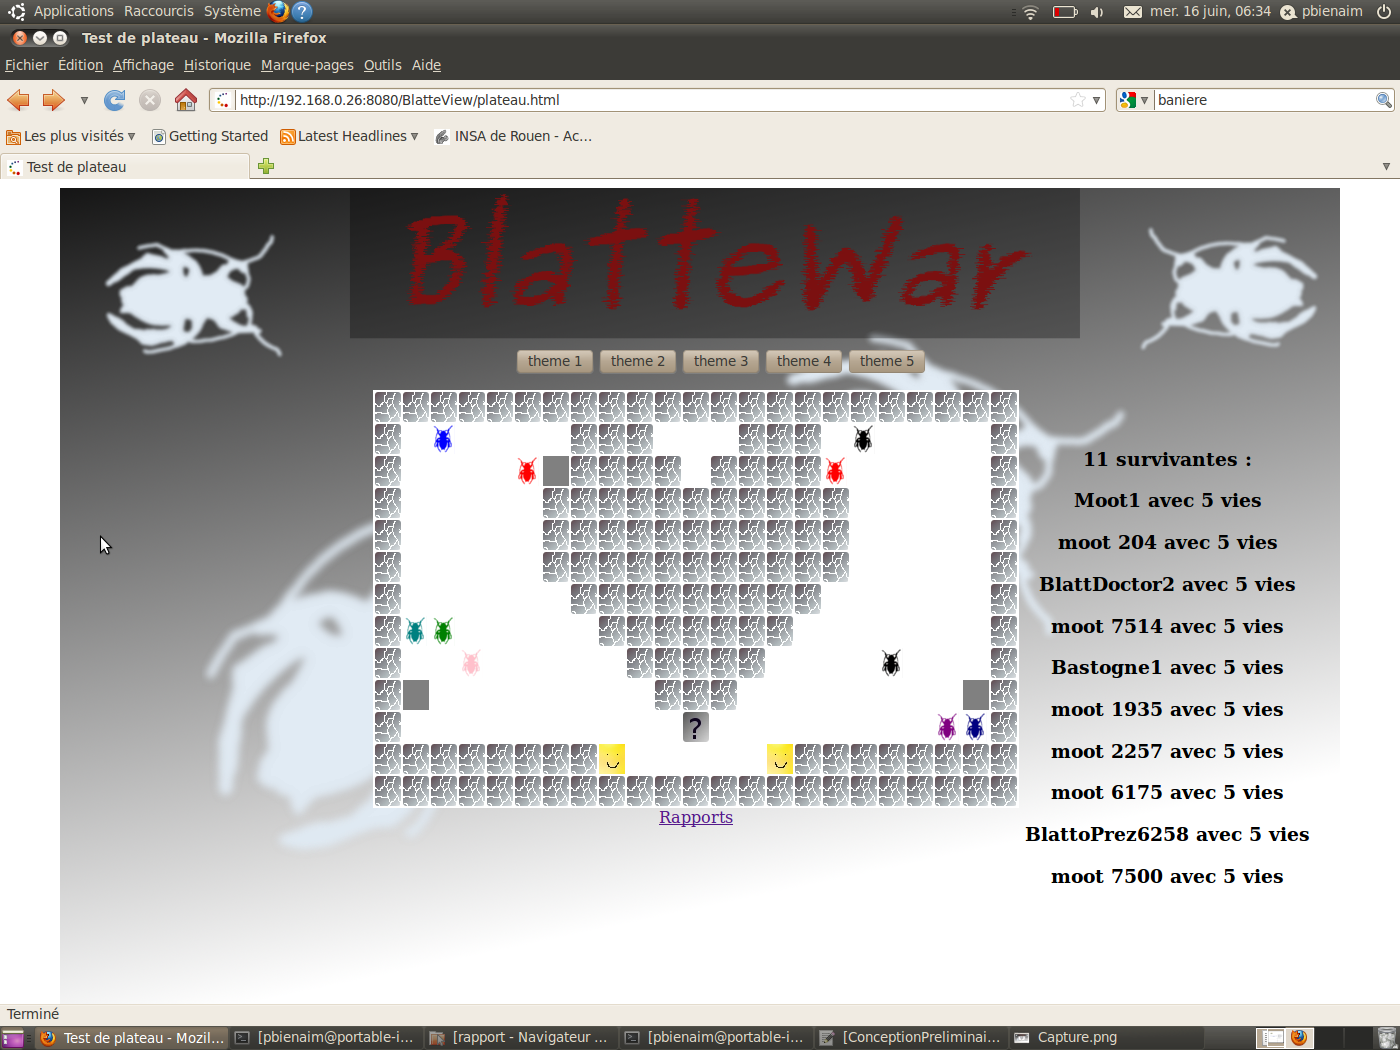
\includegraphics[width=.8\linewidth]{images/screenshot1.png}
\caption{Arène d'une partie en cours}
\end{center}
\end{figure}

    ~
    
    Enfin, il est possible de consulter les rapports complets de tous les matchs effectués, avec le détail de chaque action effectue par chaque blatte. Voici par exemple un extrait d'un rapport.
    
   \begin{figure}[h!]
\begin{center}
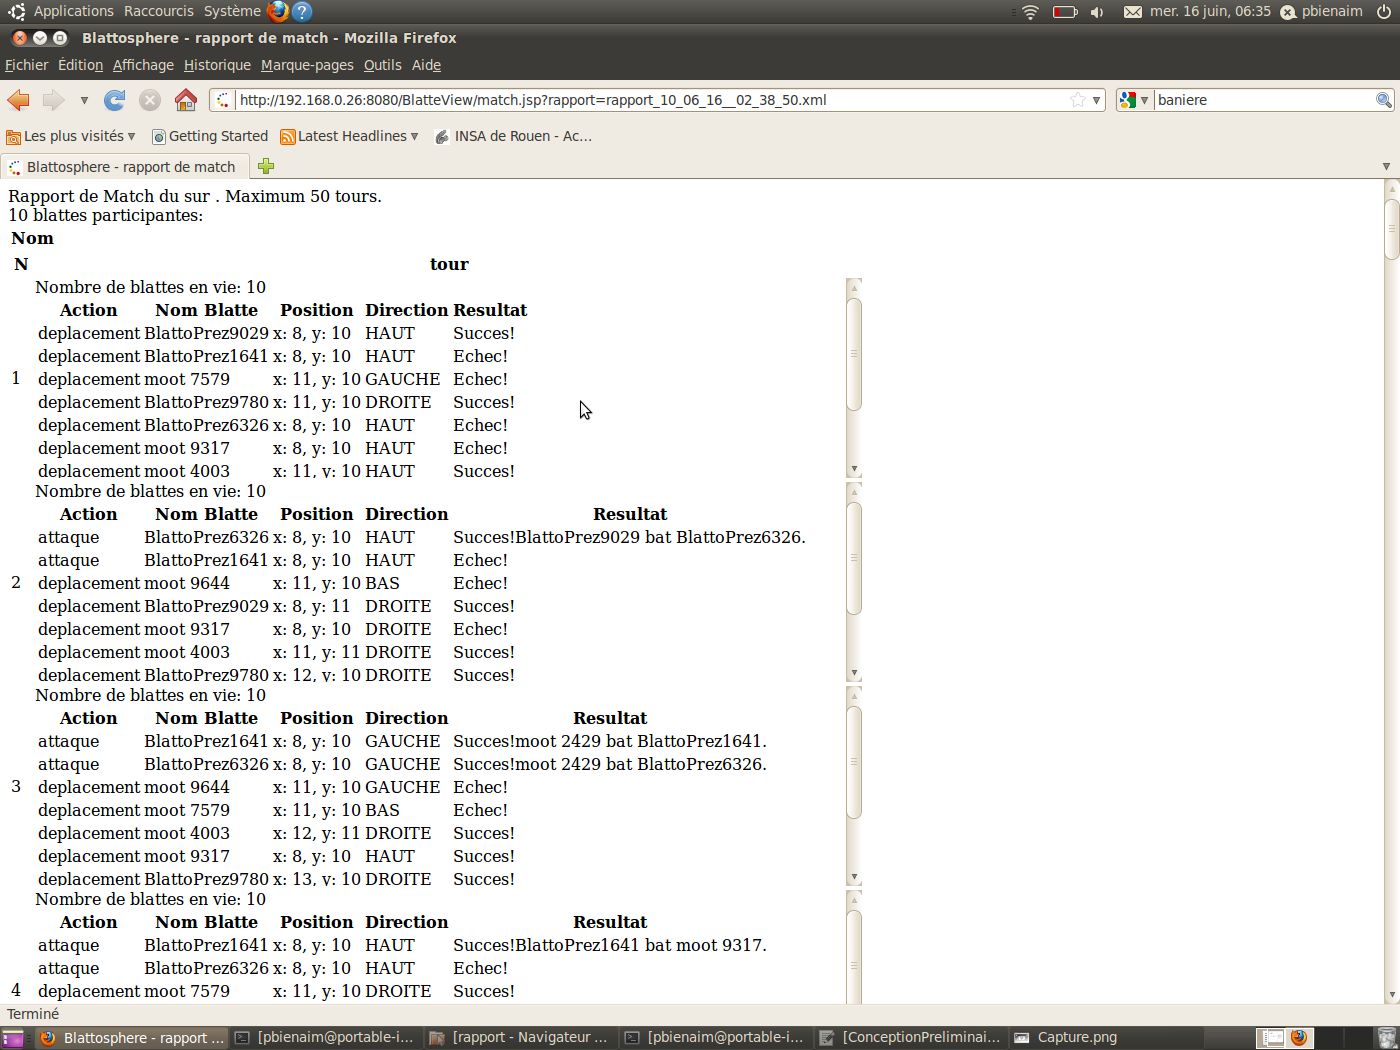
\includegraphics[width=.8\linewidth]{images/screenshot2.png}
\caption{Visualisation d'un rapport}
\end{center}
\end{figure}

 
